\documentclass{article}

\usepackage[T1]{fontenc}
\usepackage[polish]{babel}
\usepackage[utf8]{inputenc}
\usepackage{graphicx}
\usepackage{subcaption} 
\usepackage[margin=2cm]{geometry}
\usepackage{listings}
\usepackage{color}
\usepackage{amsmath}
\usepackage{tcolorbox}

\definecolor{red}{RGB}{245, 63, 60}
\definecolor{blue}{RGB}{59, 69, 245}
\definecolor{green}{RGB}{59, 245, 117}
\definecolor{yellow}{RGB}{245, 207, 59}

\title{Raport Zadanie NUM3}
\date{17.11.2023}
\author{Tomasz Dziób}

\begin{document}
  \maketitle
  \newpage
  \section{Wstęp techniczny}
  Poniższy raport dotyczy zadania numerycznego NUM3 z listy 2. Załączony program o nazwie \textit{num3.cpp} został napisany w języku \textit{C++}, do sprawdzenia obliczeń został użyty plik \textit{check.cpp} również napisany w języku \textit{C++} z wykorzystaniem bibioteki \textit{GSL}. Aby uzyskać wykres prezentujący zależność wielkości danych wejściowych od czasu dla algorytmu z zadania \textit{num3.cpp} służy plik \textit{plot.cpp} napisany języku \textit{C++} korzystający z bibioteki \textit{GNU Plot}. Przed skompilowaniem programu należy zainstalować powyższe biblioteki.

    \subsection{Jak uruchomić program?}
    Razem z załączonymi plikami znajdziemy \textit{Makefile} który służy do
    uruchomienia programu \textit{num3.cpp} oraz \textit{check.cpp} komendą: \textit{make run}.\\
    Aby uruchomić program \textit{plot.cpp} korzystamy z komendy: \textit{make runplot DATA\textunderscore AMOUNT $=$ rozmiar},\\
    gdzie \textit{rozmiar} to maksymalny rozmiar macierzy, \textit{rozmiar}  > 50

  \section{Nakreślenie problemu}
  Najwiekszą przeszkodą w rozwiązywaniu równań macierzowych jest przechowywanie danych w pamięci. Macierze dla nawet stosunkowo nie dużych zestawów danych (patrząc z perspektywy tego ile danych jest procesowanych w obecnych czasach) potrafią zajmować ogromną ilość miejsca na dysku.
  \begin{flushleft}
    Dla $N = milion$:
  \end{flushleft}

  \begin{center}
    8bajtów $\cdot N^2$ = 8 $\cdot (10^6)^2$ = 8 $\cdot 10^{12}$ bajtów = 8 $\cdot 10^3$ GB
  \end{center}
  Jednak w przypadku zadania \textit{NUM3} mamy doczynienia z macierzą tak zwaną wstęgową. Charakteryzuje się ona tym, że posiada wartości jedynie na diagonali oraz na pasmach, pod oraz nad diagonalą (liczba pasm pod oraz nad mogą być różne! - tak jak jest w tym przypadku). Pozostałe elementy są wypełnione zerami.
  
  \begin{center}
    
    
    \begin{minipage}[t]{0.14\textwidth} % Adjust the width as needed
    \hspace{0.05cm} m\\
    $\overbrace{}$ 
    \end{minipage}

    \begin{minipage}{0.3\textwidth}

      \raisebox{1.2cm}{n\{ } 
    $\begin{bmatrix}
                  \textcolor{red}{\bullet}	&	\textcolor{green}{\bullet}	&	\textcolor{yellow}{\bullet}	\\
                  \textcolor{blue}{\bullet}	&	\textcolor{red}{\bullet}	&	\textcolor{green}{\bullet}	&	\textcolor{yellow}{\bullet}	\\
      &		        \textcolor{blue}{\bullet}	&	\textcolor{red}{\bullet}	&	\textcolor{green}{\bullet}	&	\textcolor{yellow}{\bullet}	\\
      & &		      \ddots	&	\ddots	&	\ddots	&	\ddots	\\
      & & &		    \textcolor{blue}{\bullet}	&	\textcolor{red}{\bullet}	&	\textcolor{green}{\bullet}	&	\textcolor{yellow}{\bullet}	\\
      & & & &	    \textcolor{blue}{\bullet}	&	\textcolor{red}{\bullet}	&	\textcolor{green}{\bullet}	&	\textcolor{yellow}{\bullet}	\\
      & & & & &  	\textcolor{blue}{\bullet}	&	\textcolor{red}{\bullet}	&	\textcolor{green}{\bullet}	\\
      & & & & & &	\textcolor{blue}{\bullet}	&	\textcolor{red}{\bullet}	\\
    \end{bmatrix}$
  \end{minipage}
  \end{center}
  Przypadek ten pozwala nam zaoszczędzić pamięć pomijając zapisywanie zer. Można to osiągnąć poprzez trzymanie macierzy w tablicy zawierającej tylko wypełnione pasma. Rozważając ponownie poprzedni przykład:
  \begin{flushleft}
    Dla $N = milion$:
  \end{flushleft}

  \begin{center}
    8bajtów $\cdot$ $4N$ = $32N$ = 32 $\cdot$ $10^{6}$ bajtów = 32 MB
  \end{center}
  Jak zauważamy jest to diametralna różnica jeśli chodzi o zużycie pamięci.\\
  Jednakże jako, że liczba naszych danych wejściowych jest mniejsza, zmniejsza się również złożoność obliczeniowa. Jest to ogromną zaletą ponieważ standardowo dla rozwiązania układów równań liniowych jest to rząd wielkości O($N^3$), tymczasem
  dla macierzy wstęgowych tą metodą jesteśmy wstanie to rozwiązać w czasie O($N$).

  \section{Użyta metoda}
  Rozwiązanie sprowadza się do obliczenia rokładu \textit{LU} macierzy \textit{A} oraz obliczenia dwóch równań \textit{Lt = x} (metodą \textit{forward substitution}) oraz \textit{Uy = t} (metodą \textit{back substitution}) które wynikają z prostych przekształceń zadanego równania oraz podstawienia.\\
  Do osiągnięcia rozkładu \textit{LU} macierzy użyte zostały uproszczone wzory na uzyskanie poszczególnych elementów \textit{LU} (uproszczone ponieważ niektóre fragmenty uległy skróceniu przez wartości zerowe w macierzy).
  \begin{center}
    {\Large $u_{i,i} = a_{i,i} - l_{i,i-1} \cdot u_{i-1,i}$} \qquad \qquad
    {\Large $u_{i,i+1} = a_{i,i+1} - l_{i,i-1} \cdot u_{i-1,i+1}$} \\
    {\Large $u_{i,i+2} = a_{i,i+2}$} \qquad \qquad
    {\Large $l_{i+1,i} = \frac{a_{i+1,i}}{u_{i,i}}$}
  \end{center}

  \section{Uzyskany wynik}
  Po wykonaniu komendy \textit{make run} wykonają się dwa programy jeden po drugim. Najpierw otrzymamy wynik uzyskany omówioną wcześniej metodą a później obliczony z pomocą bibioteki \textit{GSL}.
    \begin{flushleft}
      $\bullet$ Plik \textit{num3.cpp}
    \end{flushleft}

    \begin{center}
      \begin{tcolorbox}
        Wektor y:\\
        0.448701 1.41327 2.13488 2.86901 3.59149 4.3116 5.02983 5.74701 6.4635 7.17953 7.89521 8.61065 9.3259 10.041 10.756 11.4709 12.1857 12.9005 13.6152 14.3299 15.0445 15.7591 16.4736 17.1882 17.9027 18.6172 19.3317 20.0462 20.7606 21.4751 22.1895 22.9039 23.6184 24.3328 25.0472 25.7616 26.476 27.1903 27.9047 28.6191 29.3335 30.0478 30.7622 31.4765 32.1909 32.9053 33.6196 34.3339 35.0483 35.7626 36.477 37.1913 37.9056 38.62 39.3343 40.0486 40.763 41.4773 42.1916 42.9059 43.6203 44.3346 45.0489 45.7632 46.4775 47.1919 47.9062 48.6205 49.3348 50.0491 50.7634 51.4777 52.1921 52.9064 53.6207 54.335 55.0493 55.7636 56.4779 57.1922 57.9065 58.6208 59.3351 60.0494 60.7637 61.478 62.1924 62.9067 63.621 64.3353 65.0496 65.7639 66.4782 67.1925 67.9068 68.6211 69.3354 70.0497 70.764 71.4783 72.1926 72.9069 73.6212 74.3355 75.0498 75.7641 76.4784 77.1927 77.9069 78.6212 79.3355 80.0498 80.7641 81.4784 82.1927 82.907 83.6213 84.3356 85.0499 85.7642 86.4785 87.1928 87.9078 88.682 
        \\
        Wyznacznik macierzy A:\\
        6.14197e+09
      \end{tcolorbox}

      \begin{flushleft}
        $\bullet$ Plik \textit{check.cpp}
      \end{flushleft}

      \begin{tcolorbox}
        Wektor y:\\
        0.448701 1.41327 2.13488 2.86901 3.59149 4.3116 5.02983 5.74701 6.4635 7.17953 7.89521 8.61065 9.3259 10.041 10.756 11.4709 12.1857 12.9005 13.6152 14.3299 15.0445 15.7591 16.4736 17.1882 17.9027 18.6172 19.3317 20.0462 20.7606 21.4751 22.1895 22.9039 23.6184 24.3328 25.0472 25.7616 26.476 27.1903 27.9047 28.6191 29.3335 30.0478 30.7622 31.4765 32.1909 32.9053 33.6196 34.3339 35.0483 35.7626 36.477 37.1913 37.9056 38.62 39.3343 40.0486 40.763 41.4773 42.1916 42.9059 43.6203 44.3346 45.0489 45.7632 46.4775 47.1919 47.9062 48.6205 49.3348 50.0491 50.7634 51.4777 52.1921 52.9064 53.6207 54.335 55.0493 55.7636 56.4779 57.1922 57.9065 58.6208 59.3351 60.0494 60.7637 61.478 62.1924 62.9067 63.621 64.3353 65.0496 65.7639 66.4782 67.1925 67.9068 68.6211 69.3354 70.0497 70.764 71.4783 72.1926 72.9069 73.6212 74.3355 75.0498 75.7641 76.4784 77.1927 77.9069 78.6212 79.3355 80.0498 80.7641 81.4784 82.1927 82.907 83.6213 84.3356 85.0499 85.7642 86.4785 87.1928 87.9078 88.682 
        \\
        Wyznacznik macierzy A:\\
        6.14197e+09  
      \end{tcolorbox}
    \end{center}
    Porównując oba wyniki jesteśmy wstanie identyczne wyniki w obu przypadkach.\\

    Aby sprawdzić czy algorytm jest optymalny powstał plik \textit{plot.cpp}. Uruchamia się go komendą \textit{make runplot DATA\textunderscore AMOUNT $=$ rozmiar}. Wykonuje on algorytm do zadanej liczby $N$, zaczynając od $i=50$ inkrementując również o 50. Dla uzyskania wyników odpornych na inne procesy działające w tle program wykonuje operacje dla każdego $N$ sto razy oraz uśrednia wynik. Po wykonaniu obliczeń otrzymujemy wyniki naniesione na wykres.\\
    \newpage

    \begin{figure}[!ht]
      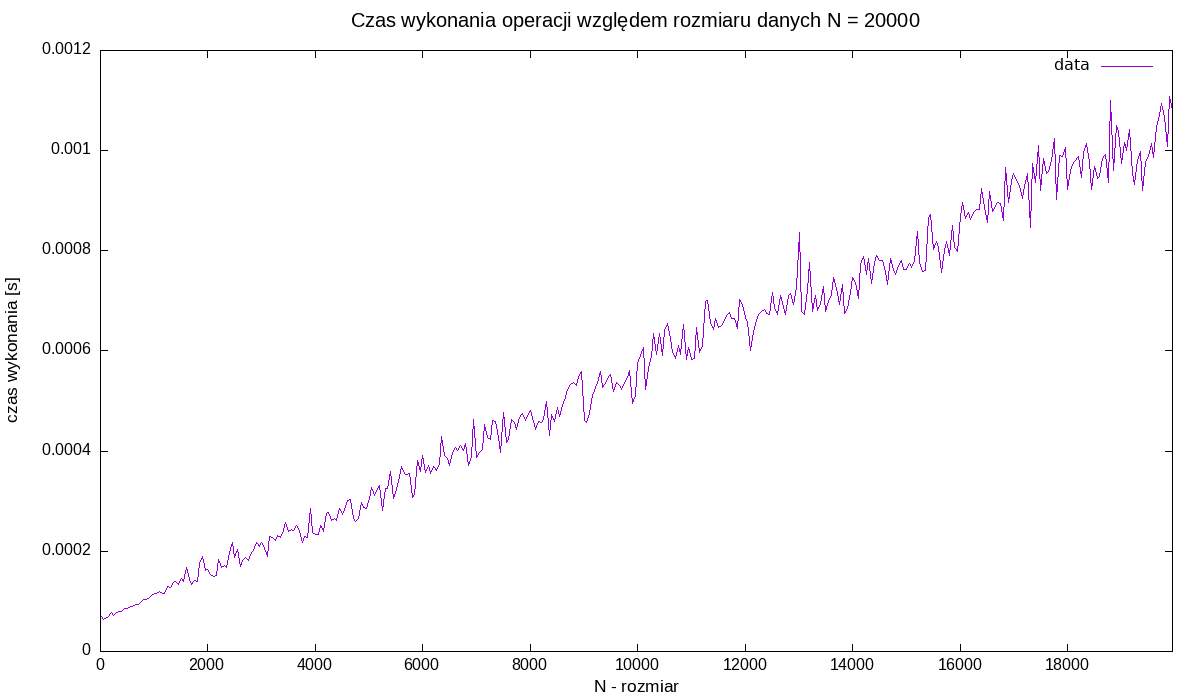
\includegraphics[width=\linewidth]{wyniki.png}
      \caption{Wynik uzyskany po uruchomienu programu \textit{plot.cpp}}
    \end{figure}

    Razem ze wzrostem rozmiaru \textit{N} jesteśmy wstanie zauważyć wzrost szumów wystepujących mimo obliczania średniej z stu uzyskanych wyników.
  \section{Podsumowanie}
    Znajomość struktury macierzy jest kluczowa przy wybieraniu odpowiedniego sposobu rozwiązania równań liniowych. Może on pozwolić na znaczne odciążenie naszego procesora ze zbędnych obliczeń poprzez zmniejszenie jego złożoności czasowej. Co więcej, właściwe dobranie sposobu przechowywania macierzy w pamięci pozwoli na rozwiązanie problemów z danymi o kilka rzędów wiekszych od dostępnego.
\end{document}